\chapter{Machine Translation}
This chapter describes the classical or start-of-the-art machine translation  (MT) models from statistical MT to neural MT. The related research work on unsupervised MT is also included.


\section{Statistical Machine Translation}
%%%
%The initial models for MT are based on words as units (Word-based MT), that can be translated, inserted, dropped and reordered.
%Fertility is the notion that input words produce a specific number of output words in the output language.
%
%Define the phrase-based statistical MT model mathematically.  First apply the Bayes rule to invert the translation direction and integrate a language model $p_{LM}$ so the best English translation for the input sentence ${f} $ is defined as 
%
%The advantages of the phrase-based MT is :
%\begin{enumerate}
%	\item many-to-many translation can handle non-compositional phrase	
%	\item better utilization of local context in translation
%	\item the more data, the longer phrases can be learned 
%\end{enumerate}
Statistical MT had achieved success in the early era of MT, until neural machine translation (NMT) emerged. The initial statistical models for MT are based on words as atomic units that may be translated, inserted, dropped and reordered. In statistical MT, we use both a translation model and a language model which encourages fluent output. Later, the statistical MT prefers to use translation of phrases as atomic units. These phrases are any contiguous sequences of words and not necessarily linguistic entities. In this approach, the input sentence is broken up into a sequence of phrases and are mapped one-to-one to output phrases, which may be reordered.

\subsection{Word-Based Model}
\noindent \textbf{Noisy-channel model}\\
Noisy-channel model is
 based on the notion of a noisy channel from Shannon's information theory, which had been applied to many language processing problems. Assuming that the source sentence is a distorted message omitted from the target sentence, we have a model on  how the message is distorted (translation model $Pr(f_1^J|e_1^I)$) and also a model on which original messages are probable (language model ${Pr(e_1^I)}$). The task is to find the best translation $\hat{e}_1^{\hat{I}}$ for an input foreign sentence.
\begin{align*}
\hat{e}_1^{\hat{I}} & = \argmax{e_1^I} \{Pr(e_1^I | f_1^J)\} \\ & = \argmax{e_1^I} {\frac{Pr(f_1^J | e_1^I)Pr(e_1^I)}{Pr(f_1^J)}} \\
& = \argmax{e_1^I} { \{ Pr(f_1^J | e_1^I) \cdot  Pr(e_1^I)\} }
\end{align*} 


\subsubsection{IBM Models}
Based on the noisy-channel model, IBM word-based translation makes the model more complicated by adding submodels. Starting from lexical translation, absolute alignment model, fertility etc. are added step by step.\\

The advances of the five IBM models are:
\begin{itemize}
	\item IBM Model 1: lexical translation;
	\item IBM Model 2: adds absolute alignment model;
	\item IBM Model 3: adds fertility model;
	\item IBM Model 4: adds relative alignment model;
	\item IBM Model 5: fixes deficiency.
\end{itemize}
 \textbf{Alignment Model} \\
 This is an explicit model for reordering words in a sentence. More often than not, words that follow each other in one language have translations  that follow each other in the output language. In detail, the position $j$ in the source sentence is aligned with the position $i$ in the target sentence when translating, denoted as  ${i=a_j}$. Alignment model is a global reordering model. For whole sentence, we denote the alignment as: 
\[a_1^J:= a_1\cdots a_J\]
There is not probabilistic model for alignment in IBM Model 1, it treats probability of all alignments equally. IBM Model 2 addresses the issue of alignment with an explicit model for alignment based on the positions of the input output words and sentence lengths $a(i|j, I, J)$. \\

\textbf{Fertility} \\
It models the specific number of output words in the output language. Generally one word in one language is just translated into one single word in the other language. But some words produce multiple words or get dropped. We denote the fertility, as $\phi(e)$.  As in all IBM models, it introduces the NULL token to account for source words that have no correspondent in target side. NULL insertion in added after the fertility step. The word-based translation process can be described as the Figure 2.1 \cite{koehn2009statistical}
\begin{figure}[t]
	\centering
	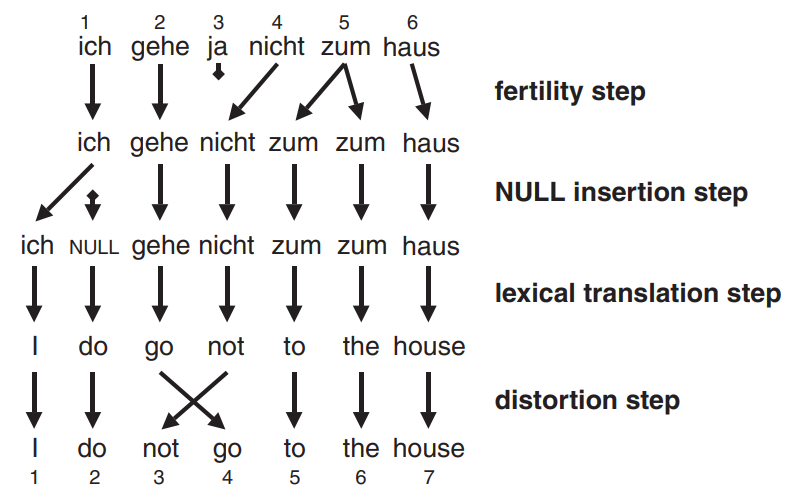
\includegraphics[width=12cm]{wordsmt}
	\caption{ Illustration of a translation process using IBM-3 model (\cite{koehn2009statistical})}

\end{figure}




\subsubsection{Weighted Model}
 In order to optimize the sub-models with appropriate weights, scaling exponents ${\lambda_{m}}$ are introduced as in speech recognition. For example,
\[ P(f_1^J, e_1^I; a_1^J) = P(J|I)^{\lambda_1} \cdot \prod_{i=1}^{I} P(e_i|e_1^{i-1})^{\lambda_2} \cdot \prod_{j=1}^{J} [P(a_j|a_{j-1}, I, J)^{\lambda_{3}} \cdot P(f_j|e_{a_j})^{\lambda_4}]  \]
where the four probabilities corresponds to length model, language model, alignment model and lexical model respectively. 


\subsection{Phrase-Based Model}
Actually when translating, words may not be the best candidates for the smallest units for translation; sometimes one word in a foreign language should be translated into two English words, or vice versa. Word-based models often break down in these cases.\\
Phrase-based models typically do not strictly follow the noisy-channel approach proposed for word-based models, but use a log-linear framework to allow s straightforward integration of additional features.\\

\textbf{Log-linear Model Combination}\\
Consider arbitrary models ("feature functions"):
\[ q_m(f_1^J, e_1^I; a_1^J) > 0  \quad m = 1, \cdots, M\]

\begin{align*}
	Q(e_1^I, f_1^J; a_1^J) & = \prod_{m=1}^{M} q_m(f_1^J, e_1^I; a_1^J)^{\lambda_m} \\
	& = \exp(\sum_{m=1}^{M} \lambda_m \log q_m(f_1^J, e_1^I; a_1^J))
\end{align*}
In this frame work, we view each data point as a vector of features and the model as a set of corresponding feature functions, these functions are trained separately and combined assuming that they are independent of each other.\\ 

Components for log-linear model can be such as language model, phrase translation model, reordering model are used as feature functions with appropriate weights.
\begin{itemize}
	\item Phrase translation model can be learned from a word-aligned parallel corpus, alternatively we also can use expectation maximization algorithm to directly find phrase alignment for sentence pairs.
	\item Reordering model for phrase case is typically modeled by a distance based reordering cost that discourage reordering in general. Lexicalized reordering model can be introduced for specific phrase pair.
\end{itemize}

The model can be further extended by components like: bidirectional translation probabilities, lexical weighting, word penalty and phrase penalty. 

\subsection{Decipherment}
\cite{ravi2011deciphering} frame the MT problem as a decipherment task, treating the foreign text as a cipher. They also propose iterative EM method and Bayesian method to train this unsupervised model. Many concepts in deciperment are the same as the SMT.\\

IBM model tries to maximize the probability with hidden alignment model
\[ \argmax{\theta} \prod_{(e_1^I,{f}_1^J) } {P_{\theta}(f_1^J|e_1^I)} = \argmax{\theta} \prod_{ (e_1^I,{f}_1^J) } \sum_{a} P_{\theta}({f}_1^J, a| e_1^I)  \]
While for unsupervised case, we train 
\[ \argmax{\theta} \prod_{f_1^J}P_{\theta}(f_1^J)= \argmax{\theta} \prod_{f_1^J} \sum_{e_1^I} P({e}_1^I) \cdot P_{\theta}(f_1^J|e_1^I)\]

for hidden alignments: \[ \argmax{\theta} \prod_{{f}_1^I} \sum_{{e}_1^I} P({e}_1^I) \cdot \sum_{a} P_{\theta}({f}_1^J,a|{e}_1^I) \]

Since the model is very complicated, more assumptions are added to the model. The model accounts for word substitutions, insertions, deletions and local reordering during the translation process but does not incorporate fertilities or global re-ordering.\\

%The generative process:
%\begin{enumerate}
%	\item Generate an English sentence $\bm{e}$ with probability $P(\bm{e})$.
%	\item Insert a NULL word at any position in the English sentence with uniform probability.
%	\item For each English word token $e_i$ (including NULLs), choose a foreign word translation $f_i$, with probability $P_{\theta}(f_i| e_i)$, the foreign word may be NULL.
%	\item Swap any pair of adjacent foreign words $f_{i-1}, f_i$, with probability ${P_{\theta}(swap)}$. 
%	\item Output the foreign string $f_1^M$, skipping over NULLs.
%\end{enumerate}
%
%However, this method is limited to rather short sentences and simplistic settings.
\section{Neural Machine Translation}
NMT has recently become the dominant method for MT task. In comparison to the traditional SMT, NMT systems are trained end-to-end, taking advantage of continuous representation of the hidden states that greatly alleviate the sparsity problem and make better use of more contextual information.Traditional phrase-based MT, which consists of several models that are tuned separately. neural MT can directly output translations given input, it contains only one single model. Also NMT models are trained with only one single training criterion. \\
\cite{sutskever2014sequence} first use a multi-layer Long Short-Term Memory (LSTM) to model a MT system. Attention mechanism has lately been used to improve neural MT by selectively focusing on parts of the source sentence during translation (\cite{DBLP:journals/corr/BahdanauCB14}, \cite{luong2015effective}). Here, inherently sequential nature precludes parallelization within training examples. Convolutional (\cite{gehring2017convolutional}) and self-attentional (\cite{vaswani2017attention}) architectures are brought forward  for significantly more parallelization during training process in order to better exploit GPU hardwares and can reach a new state-of-the-art in
translation quality.


\subsection{Encoder-Decoder Framework}
\begin{figure}[t]
	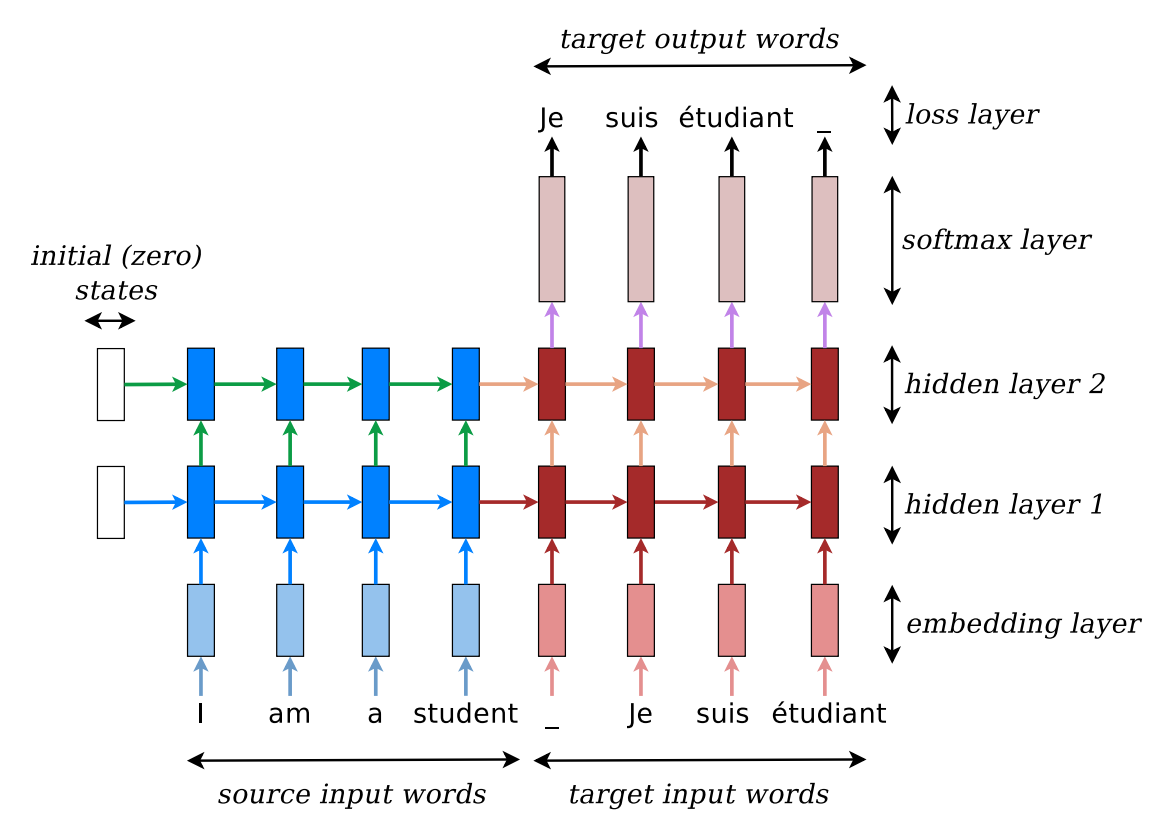
\includegraphics[width=12cm]{nmt}
	\caption{ English$\rightarrow$ French translation– example of a deep NMT (\cite{luong2015effective}).}
	\centering
\end{figure}

The most common NMT structure is the encoder-decoder framework, in which two  neural networks work together to transform one sequence to another. An encoder condenses an input sequence into a vector $\bm{c}$, and a decoder unfolds that vector into a new sequence. The model can be expressed as:
\[ p(e_1^I | f_1^J) = \prod_{i} p(e_i|e_0^{i-1}, f_1^J) = \prod_{i} {p(e_i|e_0^{i-1},  {\bm{c}})} \] 

%The final hidden and cell state from the encoder is used to initialize the state of the decoder. This means every time that the encoder model encodes an input sequence, the final internal states of the encoder model are used as the starting point for outputting the first character in the output sequence.
 The decoder predicts the next word on the basis of the internal states and the previous target words. In more detail, one can parameterize the probability of decoding each word $e_i$ as:
 \[ p(e_i|e_0^{i-1},  {\bm{c}}) = \text{softmax}(g(\bm{s_i}))\]
 with $g$ being the transformation function that outputs a vocabulary-size vector. Here $\bm{s}_i$ is the decoder hidden state, updated as:
\[ \bm{s}_i = f(\bm{s}_{i-1}, \bm{c})\]

It is common in neural MT systems to use beam search to sample the probabilities for the words in the sequence output by the model. The wider beam width leads to more exhaustive search but generally better translation quality.\\

%
%\[ p(e_t|e_{t-1} h_{t-1}, f_1^J) =  p(e_t| e_{t-1}, h_{t-1}, c_t)\]
%
%\[ \bm{\tilde{h_{t}}} = tanh(\bm{W_{c}[c_t; h_t]}) \]
%\[p(y_t| y_{<t}, x) = \text{softmax}(\bm{W_s \tilde{h_t}})\]

There are obvious drawbacks in this model that will affect the performance of translation. The model compresses all information from the input sentence into a dense vector , while ignores the length of input sentence. When the length of input sentence get very long--even longer than the training sentences, it becomes harder to extract specific information for predicting  target word for each different position. And it is not suitable to assign the same weight to all input words; one target word corresponds usually to one or several words in the input sentence. Treating all words equally does not distinguish the source information and influence the performance badly.


\subsection{Attention Mechanism}
Alignment is the problem in MT that identifies which parts of the input sequence are relevant to each word in the output, whereas translation is the process of using the relevant information to select the appropriate output.
\cite{DBLP:journals/corr/BahdanauCB14} introduce an extension to the encoder-decoder model which learns to alignment and translate jointly. Each time the model predicts the next target word, it softly searches for a set of positions in a source sentence where the most relevant information is concentrated. The model then predicts a target word based on the context vectors associated with these source positions and all the previous generated target words.\\
Described in formula, attention mechanism derives a context vector ${\bm{c}_i}$ that capture the input information to help to predict the target word at the position ${i}$. Given the target hidden state ${\bm{s}_i}$ and the source-side context vector $\bm{c}_i$, we can compute the hidden state ${\tilde{\bm{s}}_i}$ by combining the current hidden state $\bm{s}_i$ and the context vector $\bm{c_i}$:
\[ \tilde{\bm{s}}_i = tanh(W_c[\bm{c}_i; \bm{s}_i])\]

Then the target word is correspondingly predicted by softmax function:
\[  p(e_i|e_0^{i-1}, f_1^J) = softmax(W_s \tilde{\bm{s}}_i)\] 

\begin{figure}
	\centering
	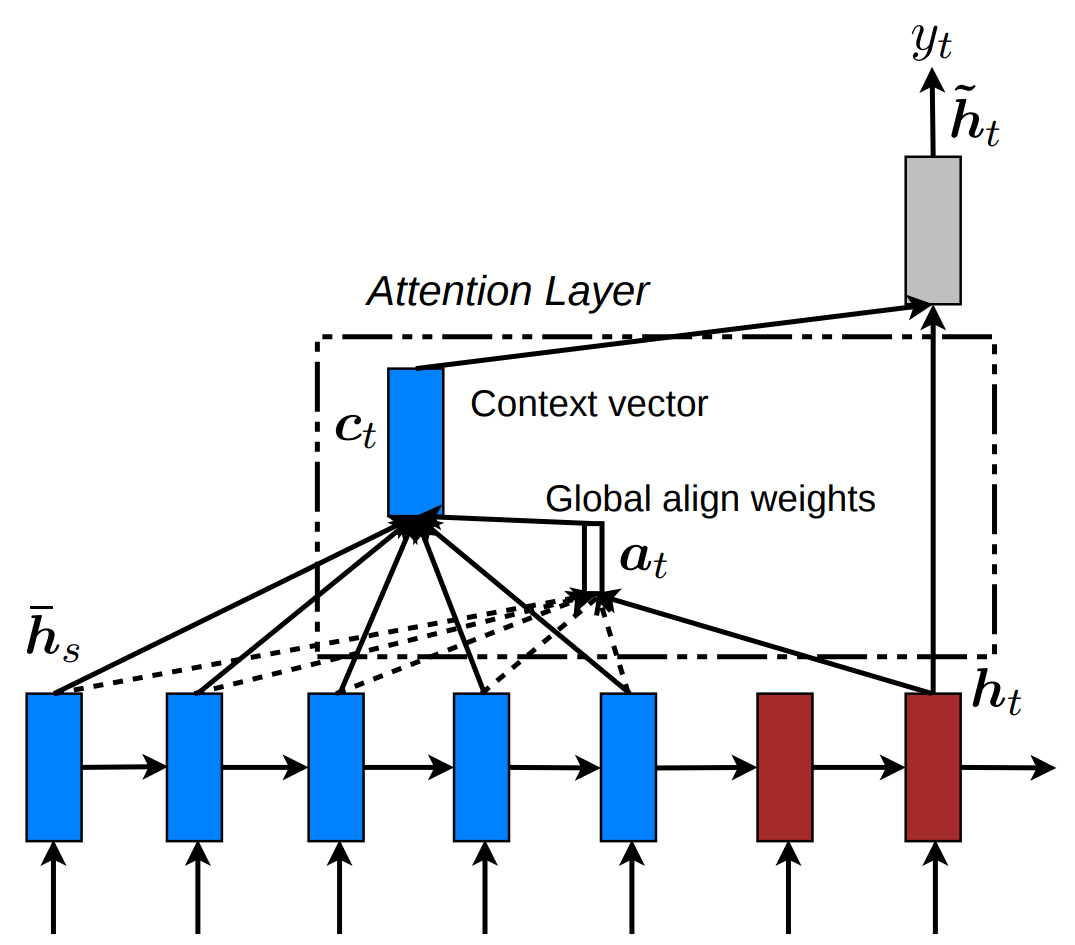
\includegraphics[width=10cm]{attentiong}
	\captionof{figure}{Global attention (\cite{luong2015effective})}	
\end{figure}
%\begin{figure}
%	\centering
%	\begin{minipage}{.5\textwidth}
%		\centering
%		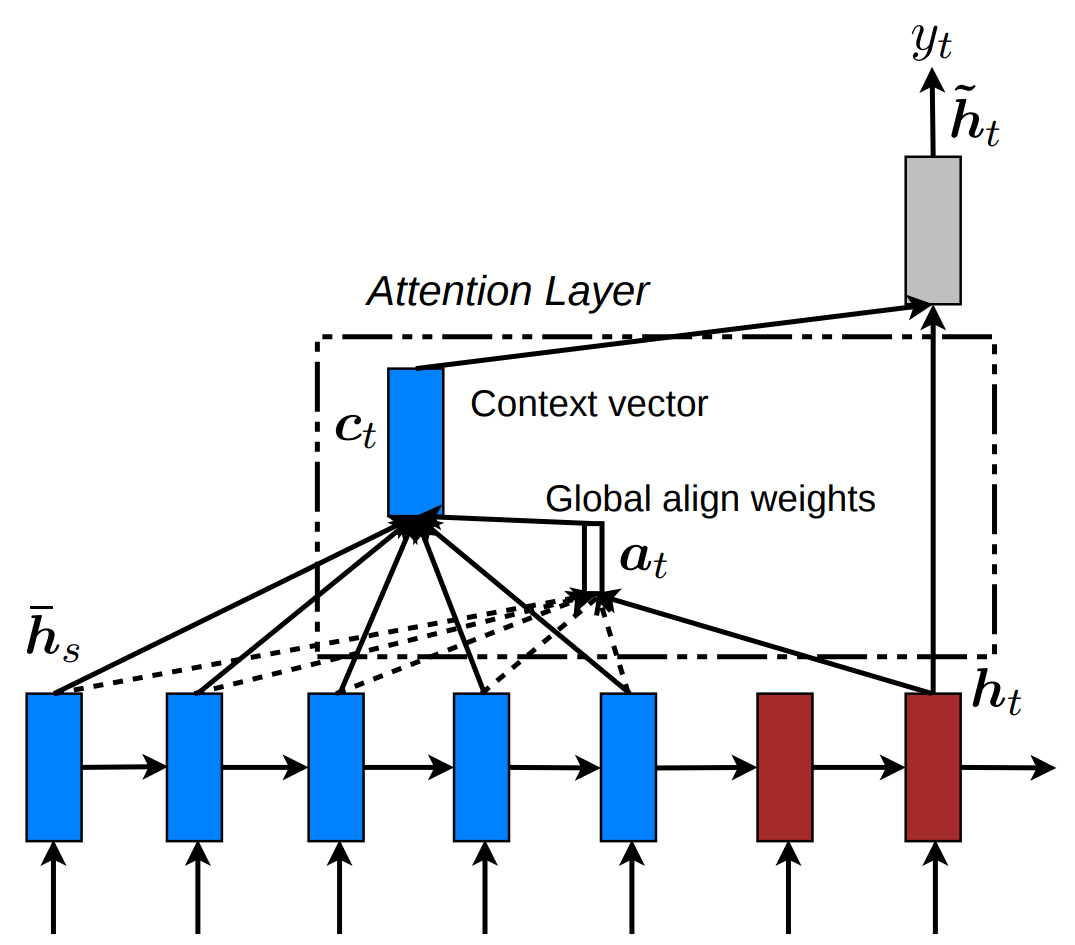
\includegraphics[width=1\linewidth]{attentiong}
%		\captionof{figure}{Global attention}
%		\label{fig:test1}
%	\end{minipage}%
%	\begin{minipage}{.5\textwidth}
%		\centering
%		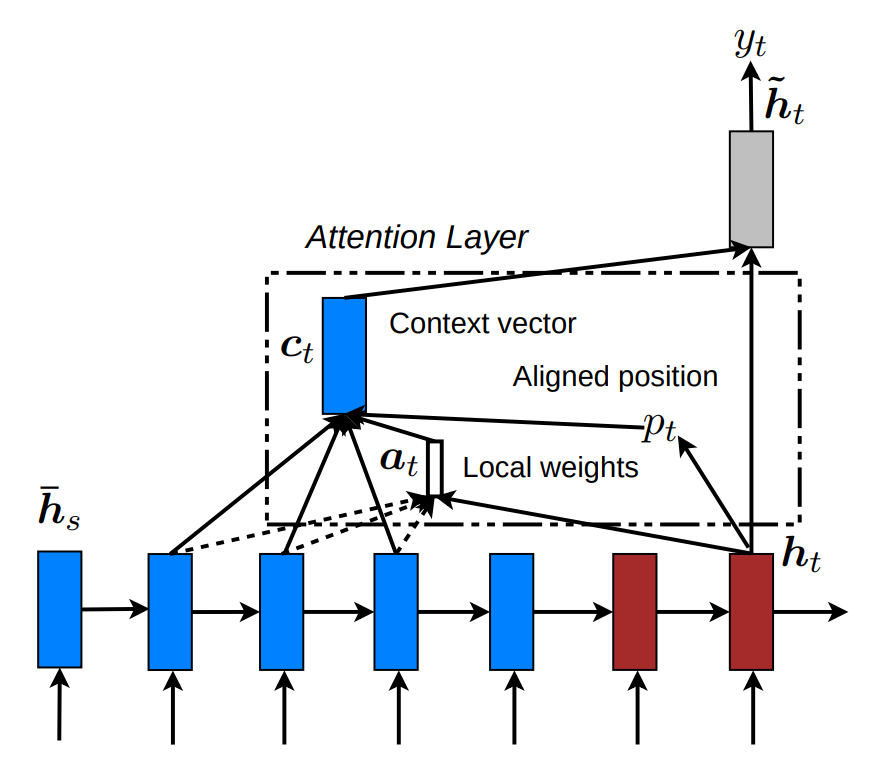
\includegraphics[width=1\linewidth]{attentionl}
%		\captionof{figure}{Local attention}
%		\label{fig:test2}
%	\end{minipage}
%\end{figure}


Attention mechanism attends all the input words, weighted average of source hidden states (word representations):
\[ \bm{c}_i = \sum_{j} {\alpha}_i(j)\cdot  \bm{h}_j \]
where $\bm{\alpha}_i(j)$ is the normalized attention weight that output at position $i$ is aligned with input position $j$, and it can be calculated as the following softmax-like function:
\begin{align}
{\alpha}_i(j) = & \ \text{align}(\bm{s}_i, {\bm{h}}_j) \\
= & \ \frac{\text{exp\ }(\text{score}(\bm{s}_i, {\bm{h}}_j))}{\sum_{\bm{j}^{\prime}} \text{exp\ }(\text{score}(\bm{s}_i, {\bm{h}}_j^{\prime}))}
\end{align}
Since score function is referred as a content based function, different forms can be considered:
\begin{equation}
\text{score}(\bm{s_i}, {\bm{h}}_j)=\left\{
\begin{array}{lcl}
{\bm{s_i}}^T {\bm{h}}_j & & dot\\
{\bm{s_i}}^T W_a {\bm{h}}_j & & general\\
{\bm{v_i}}^T tanh(W_a[\bm{s_i}; {\bm{h}}_j]) & & concat
\end{array} \right.
\end{equation}





\subsection{Transformer}

The RNN encoder-decoder models have achieved state of the art in sequence modeling and MT problem. However such RNN models also have some disadvantages, because of their inherently sequential computation which prevents parallelization across elements of the input sequence. That means it is more difficult to fully take advantage of the modern computing devices like GPU and TPU. Convolutional \cite{gehring2017convolutional} and fully-attentional feed-forward architectures like Transformer \cite{vaswani2017attention} moAnd please review your text again and find points to extend.dels are proposed as alternatives for RNNs. \\

\begin{figure}[t]
	\centering
	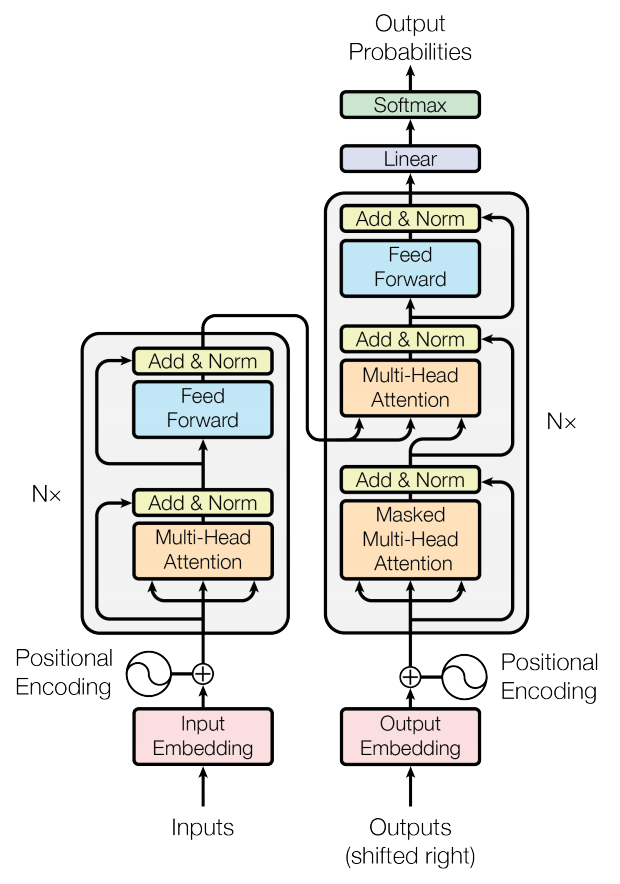
\includegraphics[width=10cm]{transformer}
	\caption{The Transformer model architecture (\cite{vaswani2017attention})}
\end{figure}
The Transformer architecture still follows the encoder-decoder framework, the encoder is composed of a stack of $N=6$ identical layers. Each layers has two sub-layers. The first is a multi-head self-attention mechanism, and the second is a simple, positionwise fully connected feed-forward network. A residual connection is employed around each of the two sub-layers, followed by layer normalization. The decoder contains also $N=6$ identical layers. In addition to the two sub-layers in each encoder layer, the decoder inserts a third sub-layer, which performs multi-head attention over the output of the encoder stack.\\
%\textbf{Dot-Product Attention}
%Given a query $\bm{q}$ and a set of key-value $(\bm{k}-\bm{v})$ pairs, the output is weighted average of values, where the weight of each value is computed by inner product of query and corresponding key. The queries and keys are of the same dimension ${d_k}$, values are of dimension ${d_v}$. Actually, for better understanding, the query $\bm{q}$  can be considered as the decoder state $\bm{s}_i$ and key $\bm{k}$ and values $\bm{v}$ can be considered as the encoder state $\bm{h}_j$ in previous attention model. Then the attention of query $\bm{q}$ on all $(\bm{k}-\bm{v})$ pairs are:
%\[ A(\bm{q}, K, V) = \sum_{i}{ \frac{\exp\ ({\bm{q}\cdot \bm{k}_i})}{\sum_{j} \exp\ {\bm{q}\cdot \bm{k}_j} } \cdot \bm{v}_i}\]
%When we stack the queries ${\bm{q}}$ to ${Q}$:
%\[ A(Q, K, V) = \text{softmax}(QK^T)V\]
%
%As ${d_k}$ get larger, the variance of ${q^T k}$ get larger.  The softmax become very peaked and the gradient get smaller. To counteract this effect, we scaled the dot products by ${\frac{1}{\sqrt{d_k}}}$, we get
%
%\[ Attention(Q,K,V) = \text{softmax}(\frac{QK^T}{\sqrt{d_k}})V\]
%The shape of resulting matrix is $n_q \times d_v$\\
\textbf{Self-Attention}\\
self-attention sublayers employs $h$ attention heads. To form the sublayer output, results from each head are concatenated and a parameterized linear transformation is applied.\\
Each attention head operates on an sequence of hidden states. For example in the encoder, given input $\bm{h}:=\bm{h}_1, \cdots \bm{h}_J$ of $J$, attention head computes a new sequence $\bm{h}^{\prime}:= \bm{h}_1^{\prime}, \cdots, \bm{h}_J^{\prime}$ of the same length.\\
Each output element, $\bm{h}_{j^{\prime}}^{\prime}$ is computed as a weighted sum of a linearly transformed input elements:
\[ \bm{h}_{j^{\prime}}^{\prime} = \sum_{{j^{\prime}}=1}^{J} \alpha_{{j^{\prime}}j}\cdot \bm{h}_{j} \]

Each weight coefficient $\alpha_{{j^{\prime}}j}$ is computed using a softmax function:
\[\alpha_{{j^{\prime}}j} = \frac{\exp {r_{{j^{\prime}}j}}}{\sum_{{\tilde{j}}=1}^{J} \exp  {r_{{j^{\prime}}{\tilde{j}}}}}\]
And $r_{{j^{\prime}}j}$ is computed using a compatibility function:
\[r_{{j^{\prime}}j} = \frac{(\bm{h}_{j^{\prime}})^{\top}(\bm{h}_j)}{\sqrt{d}} \]

\begin{figure}[h]
	\centering
	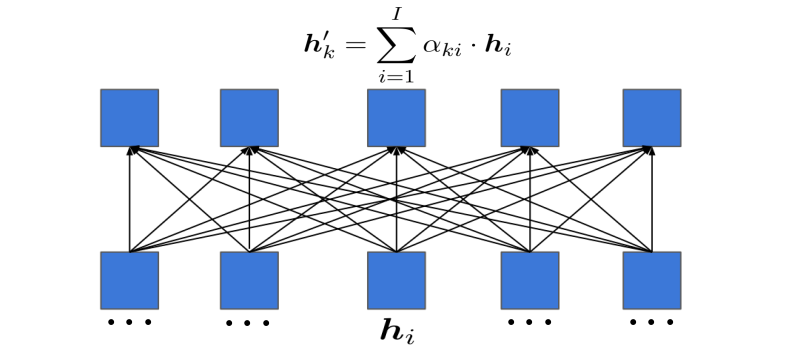
\includegraphics[width=10cm]{attentionself}
	\caption{Self-attention structure}
\end{figure}

%In the self-attention structure, the total computational complexity per layer will be greatly reduced, amount of computations can be paralellized. It performs better for long-range dependencies than traditional RNN structure.
%
%\begin{figure}[h]
%	\centering
%	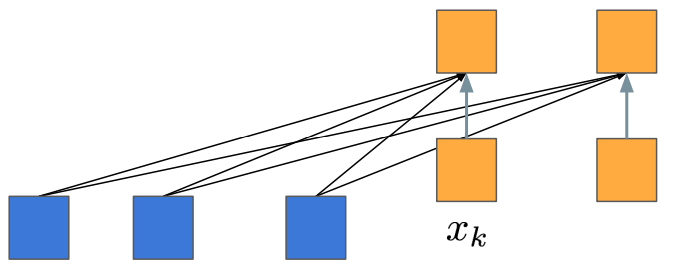
\includegraphics[width=10cm]{attentiondeen}
%	\caption{Encoder-decoder attention}
%\end{figure}

%\[ \alpha_{ki} = \frac{\exp(\text{score}(\bm{h}_k, \bm{h}_i))}{\sum_{j=1}^{I} \exp((\text{score}(\bm{h}_k, \bm{h}_j)))}\]
%\[ \text{score}(\bm{h}_k, \bm{h}_i) = \bm{h}_k^\top \bm{h}_i /\sqrt{d} , \ \ \ d= \text{dim}(\bm{h}_k)\]
%\[\bm{h}_k^{\prime} = \sum_{i=1}^{I} \alpha_{ki} \cdot \bm{h}_i\]

%\textbf{Multi-head attention}\\
% First map $Q$, $K$, $V$ into $h$ many lower dimension spaces via linear mapping matrix. Here $h$ is the number of heads. Then apply attention and concatenate the outputs. \\
%Suppose the original dimensions of queries, keys, values are ${d_{m}}$. We the number of heads is ${h}$, then we set ${d_k = d_v = d_{m}/h}$. With ${i \in 1 \cdots h}$ different matrix ${W_i^Q \in R^{d_{m}\times d_k}}$ ${W_i^K \in R^{d_{m}\times d_k}}$ ${W_i^V \in R^{d_{m}\times d_k}}$ and ${W^O \in R^{d_{m}\times d_k}}$.
%The number of attention heads in Transformers impacts their ability to capture long-distance dependencies. Especially many-headed multi-head attention is essential for modeling long-distance phenomena with only self-attention.
%\[ \text{MultiHead}(Q, K, V) = Concat(h\text{head}_1, \cdots, \text{head}_h)W^O \]
%\[\text{head}_i = Attention(QW_i^Q, KW_i^K, VW_i^V) \]
%
%where  $\text{head}_i \in \mathbb{R}^{n_q \times d_k}$,  ${\text{Multihead}(Q,K,V) \in \mathbb{R}^{n_q \times d_m}}$\\
%
%\textbf{Encoder-Decoder Attention}
%\[ \alpha_{ki} = \frac{\exp(\text{score}(\bm{s}_k, \bm{h}_i))}{\sum_{j=1}^{I} \exp((\text{score}(\bm{s}_k, \bm{f}_j)))}\]
%\[ \text{score}(\bm{s}_k, \bm{h}_i) = \bm{s}_k^\top \bm{h}_i/\sqrt{d}, \ \ \ d= \text{dim}(\bm{s}_k)\]
%%There are three attention types in the transformer model:



%\begin{itemize}
%	\item encoder-decoder attention\\
%	the queries come from the previous decoder layer, the keys and values are just the output of decoder. This works as the attention mechanism in the seq2seq model, it allow the decoder to align all positions in the input sequence with different weights
%	\item encoder self-attention\\
%	all queries, keys, values come from the encoder layer, each position allows to attend to all positions before that position
%	\item decoder self-attention\\
%	similar to encoder attention, each position is allowed to attend to position before and including that position
%\end{itemize}


%\textbf{Positional Encoding}\\
%Since there is no RNN or CNN structures in transformer model, we need also need to make use of sequence information for seq2seq learning. We need inject position information into the embedding.
%\[PE_{(\text{pos}, 2i)} = sin(\text{pos}/ 10000 ^{2i / d_{m}})\]
%\[ PE_{(\text{pos}, 2i+1)} = cos(\text{pos} / 10000^{2i/d_{m}})\]
%
%
%where pos is the position and $i$ is the dimension. That is, each dimension of the positional encoding corresponding to a sinusoid.






\subsection{Unsupervised Neural Machine Translation}
 Although the NMT systems have achieved near human-level performance on some languages, the lack of large parallel corpora poses a major challenge for many low-resource languages.
 Techniques are raised to alleviate this issue with like triangulation and semi-supervised learning techniques.  Monolingual data are leveraged to improve the quality of translation system. \\
 Recently, several neural algorithms with fully unsupervised settings are proposed. The core idea is very similar to the dual learning in MT (\cite{he2016dual}). The systems all contain bidirectional models as sub-systems, where pseudo parallel data are created with back-translation for each iteration in both translation directions. It turns the unsupervised problem into a supervised translation setting. With better translation , both sub-systems get improved synchronously.\\
 Though the dual unsupervised translation structure has achieved a relative good results, the efficiency of training such system are costly, especially because the back-translation element.
%   the end-to-end method performs better and easier to tune without much specific linguistic knowledge. The Idea is similar to dual learning framework except that in dual learning model, gradients are backpropagated through the reverse model and pretrain using a relative large parallel data as a warm start. The neural model mapping the sentences from monolingual corpora into the same latent space, By learning to reconstruct in both languages from the shared feature space. The translation model in both direction will be improved synchronously with the back-translation.




%The key idea is to build a common latent space between the two languages (or domains) and to learn to translate by reconstructing in both domains according to two principles. 



%They initialize the model with an inferred bilingual dictionary. They leverage strong language model: denoising autoencoder,  third, they implemented the back translation: the key idea is to train two translation models which translate in contrary directions at the same time. The last property is that the models constrain the latent representations produced by the encoder to be shared between the two languages. The encoders will encoder the input into a common latent representation space independent of the language. The decoder plays the role of translator and will try to learn to improve the translation quality with the help of back translation mechanism.

\textbf{Dual Structure}\\
Dual structure is inspired by the observation: any MT has a dual task: e.g. German-to-English translation (primal) and English-to-German translation (dual). Dual tasks can form a closed loop and generate informative  feedback signals to for both translation models. Based on the feedback signals generated during this process, and leverage language model, we can minimize the reconstruction error of the original sentences. We can iteratively update the two models until convergence.   \cite{he2016dual} train two agents to translate in opposite directions and make them teach each other through a reinforcement learning process. While promising, this approach still requires a parallel corpus for a warm start. \cite{lample2018phrase} simplify this structure; the gradients will not be back-propagated through the reverse model, but only make use of the back-translation. The training process is depicted in Algorithm 1 \cite{lample2018phrase}\\


\begin{algorithm}[h]
	\SetAlgoLined
	\textbf{Language models:} $\textbf{LM}_f$, $\textbf{LM}_e$ over source and target languages;\\
	\textbf{Initial translation model:}  Leveraging $\textbf{LM}_f$, $\textbf{LM}_e$, lean two initial translation models in each direction: $\Theta_{f\rightarrow e}^{(0)}$, ${\Theta_{e \rightarrow f}^{(0)}}$;\\
	\For{k = 1 to N}{
		\textbf{Back-translation:} Generate source and target sentences using the current translation models $\Theta_{f\rightarrow e}^{(k-1)}$ and $\Theta_{e\rightarrow f}^{(k-1)}$, leverading $\textbf{LM}_f$, $\textbf{LM}_e$;\\
		\textbf{Retrain:} Train new translation models $\Theta_{e\rightarrow f}^{(k)}$ and $\Theta_{f\rightarrow e}^{(k)}$ using the generated sentences and leverading $\textbf{LM}_f$, $\textbf{LM}_e$;
	}
	\caption{Unsupervised Machine Translation}
\end{algorithm}


\textbf{Initialization}\\
Without enough information to start the dual MT system, it will be hard for the system to catch meaningful signals and then it will take much more iterations. One option is to initialize the system by a naive a word-by-word translation of the sentence, where the bilingual lexicon are derived from the same monolingual data. Though such initial word-by-word translation may be poor for languages or corpora that are not closely related, it still preserves some  original semantics.\\
%\log P_{t\rightarrow t}(e|\text{noise}(e)
%\log P_{s\rightarrow s}(f|\text{noise}(f)) 


\textbf{Shared Latent Representation} \\
A shared encoder representation acts like an interlingua, which is translated into corresponding language regardless of the input source language. Since the  supervision information only comes from the monolingual data, the model learn to translate by learning to reconstruct in both language from this shared space.\\
In order to share the encoder representations, we share all encoder and decoder parameters including the embedding matrices since we perform joint tokenization across the two languages. While sharing the encoder is critical to get the model to work, sharing the decoder simply induces useful regularization.\\



\textbf{Optimization}\\
When minimizing the loss function, gradients will not be back propagated through the reverse model which generate the data. Instead the objective function minimized at every iteration is the sum of $L^{auto}$ and $L^{back}$
\begin{itemize}
	\item Denoising autoencoder loss
	\[ \mathcal{L}^{auto} = \mathbb{E}_{e_1^I \sim \mathcal{E}}[-\log P_{t\rightarrow t}(e_1^I|\text{noise}(e_1^I))] + \mathbb{E}_{f_1^J\sim \mathcal{F}} [-\log P_{f\rightarrow e}(f_1^J|\text{noise}(f_1^J))]\]
	where $s$ $P_{f\rightarrow f}$ and $P_{e\rightarrow e}$ are the probability of encoder and decoder both operating in the source and target sides, respectively
	\item Back-translation loss
	\[ \mathcal{L}^{back} = \mathbb{E}_{e_1^I\sim \mathcal{E}} [-\log P_{f\rightarrow e}(e_1^I|u(e_1^I))] +  \mathbb{E}_{f_1^J\sim \mathcal{F}} [-\log P_{e\rightarrow f}(f_1^J|v(f_1^J))]\]
	 we denote the sentence that translated by intermediate target-to-source translation model as $u(e_1^I)$, similarly denote the sentence translated by source-to-target model as $v(f_1^J)$, so $u(y)$ should in source language and $v(x)$ should in target language. The pairs $(f_1^J, v(f_1^J))$, $(u(e_1^I), e_1^I)$ constitute synthetic parallel  sentences.
\end{itemize}










